% chapter02.tex

 %%%%%%%%%%%%%%%%%%%%%%%%%%%%%%%%%%%%%%%%%%%%%%%%%%%%%%%%%%%%%%%%%%%%%%%%%%%%%
 %                                                                           %
 %    PyMS documentation                                                     %
 %    Copyright (C) 2005-8 Vladimir Likic                                    %
 %                                                                           %
 %    The files in this directory provided under the Creative Commons        %
 %    Attribution-NonCommercial-NoDerivs 2.1 Australia license               %
 %    http://creativecommons.org/licenses/by-nc-nd/2.1/au/                   %
 %    See the file license.txt                                               %
 %                                                                           %
 %%%%%%%%%%%%%%%%%%%%%%%%%%%%%%%%%%%%%%%%%%%%%%%%%%%%%%%%%%%%%%%%%%%%%%%%%%%%%

\chapter{Using PyMS}

\section{Introduction}

This chapter demonstrates main functions of PyMS in a tutorial like manner.
The data files used in the examples are provided in the project 'pyms-data'.
The commands executed interactively are grouped together by example, and
provided as Python scripts in the project 'pyms-test'.

The setup used in the examples below is as follows. The projects 'pyms',
'pyms-test', 'pyms-docs', and 'pyms-data' were downloaded in the directory
{\tt /home/current/proj/PyMS}. In the project 'pyms-test' there is a directory
corresponding to each example coded with the example number (ie.
{\tt pyms-test/01/} corresponds to Example 1). In each example directory
there is a script named 'proc.py' which contains the commands given in
the example. Provided that the paths to 'pyms' and 'pyms-data' are set
properly, these scripts could be run with the following command:

\$ python proc.py

Before running each example the Python interpreter was made aware of the
PyMS location with the following commands:

\begin{verbatim}
import sys
sys.path.append("/home/current/proj/PyMS/")
\end{verbatim}

For brevity these commands will not be shown in the examples below, but
they are included in 'pyms-test' example scripts.  The above path need
to be adjusted to match your own location of pyms.

All data files (raw data files, peak lists etc) used in the example below
can be found in 'pyms-data'.


\section{Example 1: Reading of GC-MS data and basic manipulation of
data}

\subsection{Reading ChemStation GC-MS data into PyMS}

\noindent
{\em This example is in pyms-test/01}

The PyMS package pyms.IO provides capabilities to read the raw GC-MS
data stored in the ANDI-MS format. The function IO.ANDI.ChemStation()
provides the interface to ANDI-MS data files saved from Agilent
ChemStation software.\footnote{ANDI-MS data format stands for Analytical
Data Interchange for Mass Spectrometry, and was developed for the
description of mass spectrometric data developed in 1994 by Analytical
Instrument Association. ANDI-MS is essentially a recommendation, and
it is up to individual vendors of mass spectrometry processing software
to implement "export to ANDI-MS" feature in their software.}

The file 'a0806\_140.CDF' is a GC-MS experiment exported from Agilent
ChemStation (located in 'pyms-data'). This file can be loaded in the
memory as follows:

\begin{verbatim}
>>> from pyms.IO.ANDI.Class import ChemStation
>>> andi_file = "/home/current/proj/PyMS/pyms-data/a0806_140.CDF"
>>> andi_data = ChemStation(andi_file)
 -> Processing netCDF file '/home/current/proj/PyMS/pyms-data/a0806_140.CDF'
    [ 3236 scans, masses from 50 to 550 ]
>>>
\end{verbatim}

\noindent
The above command creates the object 'andi\_data' which is an {\em instance}
of the class IO.ANDI.ChemStation.

\subsection{Exploring an ANDI-MS data object}

The object 'andi\_data' has several attributes and methods associated with it.

\begin{verbatim}
>>> print "ANDI-MS data filename:", andi_data.get_filename()
ANDI-MS data filename: /home/current/proj/PyMS/pyms-data/a0806_140.CDF
\end{verbatim}

The method {\tt get\_tic()} return total ion chromatogram (TIC) of the data
as an IonChromatogram object:

\begin{verbatim}
tic = andi_data.get_tic()
\end{verbatim}

\noindent
An IonChromatogram object is a one dimensional vector containing
mass intensities as a function of retention time. This can can be either
m/z channel intensities (for example, ion chromatograms at m/z = 65),
or cumulative intensities over all measured m/z (TIC).

The method {\tt get\_ic\_at\_index(i)} returns i-th ion chromatogram, as
an IonChromatogram object. For example, to get the first ion chromatogram
from the data:

\begin{verbatim}
ic = andi_data.get_ic_at_index(1)
\end{verbatim}

The method {\tt get\_ic\_at\_mass(MZ)} returns the ion chromatogram for
m/z = MZ.  For example, to get the ion chromatogram that corresponds
to m/z = 73:

An ion chromatogram object has a method {\tt is\_tic()} which returns
True is the ion chromatogram is TIC, False otherwise:

\begin{verbatim}
>>> print "'tic' is a TIC:", tic.is_tic()
'tic' is a TIC: True
>>> print "'ic' is a TIC:",ic.is_tic()
'ic' is a TIC: False
\end{verbatim}

\subsection{Writing data to a file}

The method {\tt write()} of IonChromatogram object allows one to save
the ion chromatogram object to a file:

\begin{verbatim}
>>> tic.write("output/tic.dat", minutes=True)
>>> ic.write("output/ic.dat", minutes=True)
\end{verbatim}

\noindent
The flag minutes=True indicates that retention time will be saved in minutes.
The ion chromatogram object saved with with the {\tt write{}} method is a
plain ASCII file which contains a pair of (retention time, intensity) per
line:

\begin{verbatim}
$ head tic.dat
  5.0944      745997.0000
  5.1002      726566.0000
  5.1059      717704.0000
  5.1116      684214.0000
  5.1173      701866.0000
  5.1230      893306.0000
  5.1287     1278099.0000
  5.1345     1290984.0000
  5.1402      925558.0000
  5.1459      644122.0000
\end{verbatim}

\noindent
Figure \ref{tic-plot} shows the plot of the file 'tic.dat' produced with the
program Gnuplot. The Gnuplot script used to produce this plot is provided
as pyms-test/01/output/plot.gnu.

\begin{figure}[htp]
\begin{center}
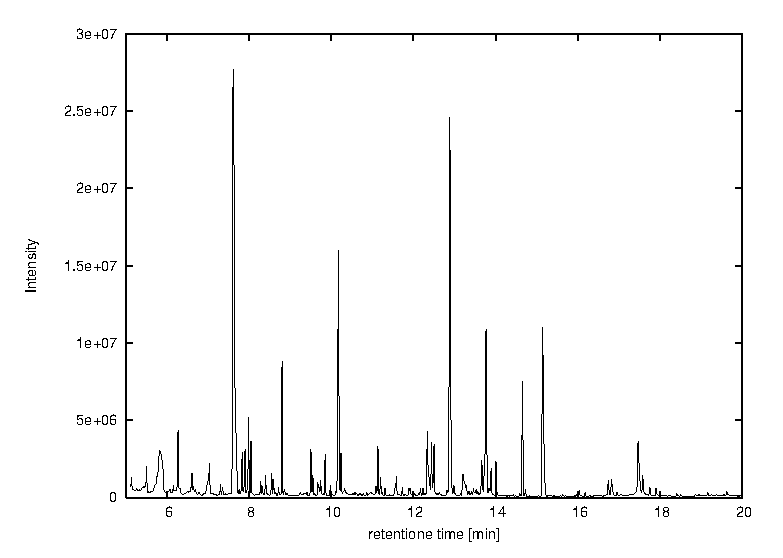
\includegraphics{graphics/tic.eps}
\caption{The Gnuplot plot of the file 'tic.dat'}
\label{tic-plot}
\end{center}
\end{figure}

The method {\tt get\_intensity\_matrix()} of ChemStation object returns
the entire matrix of intensities:

\begin{verbatim}
>>> im = andi_data.get_intensity_matrix()
>>> print "Dimensions of the intensity matrix are:",len(im),"x",len(im[0])
Dimensions of the intensity matrix are: 3236 x 501
\end{verbatim}

\noindent
This data matrix contains 3236 time points (MS scans), and each time point
corresponds to a mass spectrum of 501 m/z points.

The intensity matrix can be saved to a file with the function 'save\_data()':

\begin{verbatim}
save_data("output/im.dat", im)
\end{verbatim}

The entire data (ie. ChemStation object) can be saved as CSV with the method
{\tt export\_csv()}. For example,

\begin{verbatim}
>>> andi_data.export_csv("output/data")
\end{verbatim}

\noindent
will create 'data.im.csv, data.mz.csv, and data.rt.csv where these are the
intensity matrix, retention time vector, and m/z vector in the CSV format.

\section{Example 2: Creating signal peaks}

\noindent
{\em This example is in pyms-test/02}
G
In PyMS a signal peak is represented as 'Peak' object defined in
pyms.Peak.Class.py. A peak object is initialized with two arguments:
peak retention time and peak raw area. The following commands create
a peak named 'p' with the retention time of 5.553 min and a peak area
of 2759280 (this is the peak no. 3 in the ChemStation peak area report
file 'a0806\_140.txt'):

\begin{verbatim}
>>> from pyms.Peak.Class import Peak
>>> p = Peak(5.553*60.0,2759280)
\end{verbatim}

\noindent
As a matter of convention PyMS internally stores retention times in seconds,
hence above the retention time is multiplied by 60. Peak raw area is in
arbitrary units.

Peak properties can be accessed through its attributes:

\begin{verbatim}
>>> print "Peak retention time is", p.rt
Peak retention time is 333.18
>>> print "Peak raw area is", p.raw_area
Peak raw area is 2759280.0
\end{verbatim}

\noindent
Other important properties of a peak object are peak normalized area
and peak mass spectrum. The peak created in the above example does
not have values associated with these two attributes, and they are
merely initialized to 'None':

\begin{verbatim}
>>> print "Peak normalized area is", p.norm_area
Peak normalized area is None
>>> print "Peak mass spectrum is", p.mass_spectrum
Peak mass spectrum is None
\end{verbatim}

\noindent
The peak mass spectrum can be set by calling the method {\tt set\_mass\_spectrum()}.
This method requires the raw data, and fetches mass spectrum at peak
retention time:

\begin{verbatim}
>>> p.set_mass_spectrum(andi_data)
\end{verbatim}

\noindent
This will set the mass spectrum attribute: 

\begin{verbatim}
>>> print p.mass_spectrum
 49976  54520 102752  15570   1872  18392   8765  14966  46136  16141
  1635   1743    686   1019    712   1199   1641   3182   1234  30400
  4261   3746   3348  82392   8354  24824   3797   6086  23312 140480
[--output deleted--]
\end{verbatim}

\noindent
These are m/z channel intensities in arbitrary units. The m/z values
themselves are in the mass list attribute:

\begin{verbatim}
>>> print p.mass_list
[50, 51, 52, 53, 54, 55, 56, 57, 58, 59, 60, 61, 62, 63, 64, 65,
66, 67, 68, 69, 70, 71, 72, 73, 74, 75, 76, 77, 78, 79, 80, 81,
[--outout deleted--]
\end{verbatim}

\noindent
The length of the two arrays must match:

\begin{verbatim}
>>> print len(p.mass_spectrum)
501
>>> print len(p.mass_list)
501
\end{verbatim}

The mass spectrum can be written to a file by calling the peak
{\tt write\_mass\_spectum()} method:

\begin{verbatim}
>>> p.write_mass_spectrum("output/ms.dat")
\end{verbatim}

\noindent
The file 'output/ms.dat' contains the pairs (mz, intensity), one pair
per line:

\begin{verbatim}
$ head output/ms.dat
  50.000        49976.000
  51.000        54520.000
  52.000       102752.000
  53.000        15570.000
  54.000         1872.000
  55.000        18392.000
  56.000         8765.000
  57.000        14966.000
  58.000        46136.000
  59.000        16141.000
\end{verbatim}

Figure \ref{mass-spectrum} shows the plot of ms.dat created with the
program Gnuplot. The gnuplot script used to create this plot is
provided as pyms-test/02/output/plot.gnu.

\begin{figure}[htp]
\begin{center}
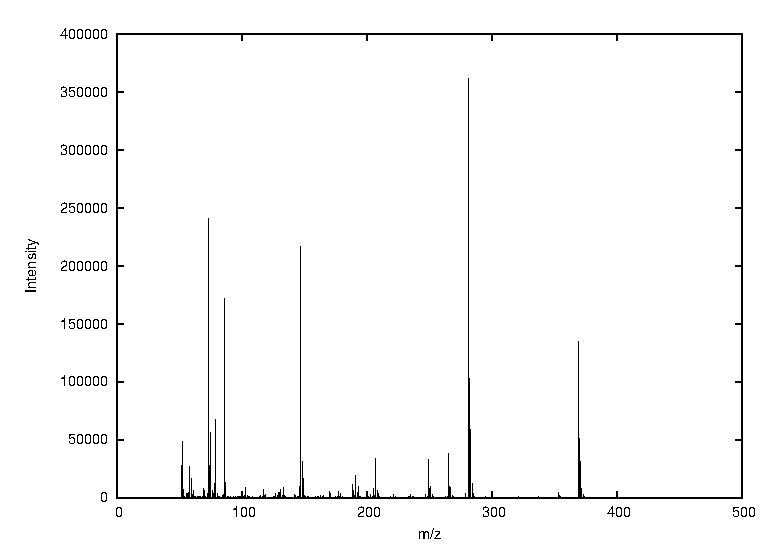
\includegraphics{graphics/ms.eps}
\caption{The plot of the file 'ms.dat' produced with Gnuplot}
\label{mass-spectrum}
\end{center}
\end{figure}

\section{Example 3: Creating an experiment from ChemStation data}

\noindent
{\em This example is in pyms-test/03}

The input files used in this example are 'a0806\_140.CDF' (ANDI-MS data
file exported from Agilent ChemStation) and 'a0806\_140.txt.a' (the 
corresponding peak area report file generated by ChemStation).

The original peak area report file exported from ChemStation is
'a0806\_140.txt'. This file was manually edited to flag non-informative
peaks, and also peaks which originate from internal reference compounds
added during the sample preparation. For example, below is the snippet
of the original file 'a0806\_140.txt':

\begin{verbatim}
 52   8.215   470  478  480 PV 3   91906   1414873   0.14%   0.056%
 53   8.242   480  483  486 VV 4   99010   1301807   0.13%   0.051%
 54   8.285   486  490  495 VV 2  124626   2241940   0.22%   0.088%
 55   8.337   495  499  501 VV 2   44820    662145   0.06%   0.026%
 
 56   8.365   501  504  506 VV 2   58181    789953   0.08%   0.031%
 57   8.399   506  510  515 VV    713172   9893695   0.97%   0.389%
 58   8.443   515  518  521 VV 5  143812   2590885   0.25%   0.102%
 59   8.477   521  524  526 VV 4  149127   2438042   0.24%   0.096%
 60   8.548   526  536  558 VV 2 55398426 1025005618 100.00%  40.335%
\end{verbatim}

\noindent
and the same file in the file 'a0806\_140.txt.a'

\begin{verbatim}
 52   8.215   470  478  480 PV 3   91906   1414873   0.14%   0.056%
 53   8.242   480  483  486 VV 4   99010   1301807   0.13%   0.051% BLANK
 54   8.285   486  490  495 VV 2  124626   2241940   0.22%   0.088%
 55   8.337   495  499  501 VV 2   44820    662145   0.06%   0.026%
 
 56   8.365   501  504  506 VV 2   58181    789953   0.08%   0.031%
 57   8.399   506  510  515 VV    713172   9893695   0.97%   0.389%
 58   8.443   515  518  521 VV 5  143812   2590885   0.25%   0.102%
 59   8.477   521  524  526 VV 4  149127   2438042   0.24%   0.096%
 60   8.548   526  536  558 VV 2 55398426 1025005618 100.00%  40.335% BLANK
\end{verbatim}

\noindent
In the file 'a0806\_140.txt.anno' the keywork 'BLANK' was manually added to peaks
53 and 60, which are known to originate from the derivatizing agent use in GC-MS
data preparation.  These peaks can be excluded from the analysis later.

The peak eluting at 15.590 min originated from scyllo-inositol reference
compound added during sample preparation. In the file 'a0806\_140.txt.anno'
this peak was labelled as follows:

\begin{verbatim}
178  15.590  1758 1767 1773 VV   5307268  80504143   7.85%   3.168% RF-SI
\end{verbatim}

\noindent
There could be an arbitrary number of reference peaks in the peak list, and each
must have a unique reference 'tag' starting with 'RF-' and following with a two
letter code denoting a particular reference compound (in this case SI for
scyllo-inositol).

The ChemStation peak list is loaded in PyMS with the function
'read\_chem\_station\_peaks()':

\begin{verbatim}
>>> from pyms.Peak.List.IO import read_chem_station_peaks
>>> peak_file = "/home/current/proj/PyMS/pyms-data/a0806_140.txt.anno"
>>> peaks = read_chem_station_peaks(peak_file)
 -> Reading ChemStation peak integration report
'/home/current/proj/PyMS/pyms-data/a0806_140.txt.anno'
\end{verbatim}

\noindent
The variable 'peaks' now contains the peaks from the file 'a0806\_140.txt.a'
This is merely a Python list:

\begin{verbatim}
>>> type(peaks)
<type 'list'>
>>> print "The number of peaks is:", len(peaks)
The number of peaks is: 347
\end{verbatim}

The next step is to set the mass spectrum is set for each peak. For this we need
first to load the raw data:

\begin{verbatim}
>>> import sys
>>> sys.path.append("/home/current/proj/PyMS/")
>>> from pyms.IO.ANDI.Class import ChemStation
>>> andi_file = "/home/current/proj/PyMS/pyms-data/a0806_140.CDF"
>>> andi_data = ChemStation(andi_file)
 -> Processing netCDF file '/home/current/proj/PyMS/pyms-data/a0806_140.CDF'
    [ 3236 scans, masses from 50 to 550 ]
\end{verbatim}

\noindent
The following command sets the mass spectrum for each peak,

\begin{verbatim}
>>> for peak in peaks:
...     peak.set_mass_spectrum(andi_data)
\end{verbatim}

The experiment object is initiated with the list of peaks and the experiment
label, in this case "a0806\_140":

\begin{verbatim}
>>> from pyms.Experiment.Class import Experiment
>>> expr = Experiment("a0806_140", peaks)
\end{verbatim}

\noindent
In the next steps we call a series of methods associated with the experiment
object to set the reference peak, remove blank peaks, create peak normalized
area (in this case the same as peak raw area), purge negative peaks (if
any), and finally select the retention time range for the experiment to
between 6.5 and 21 minutes, discarding all peaks outside this range:

\begin{verbatim}
>>> expr.set_ref_peak("si")
 [ Reference peak found: 'rf-si' @ 935.400 s ]
  [ Removing reference peak 'rf-si' @ 935.400 s ]
>>> expr.remove_blank_peaks()
        [ Designated blank peak at 438.660 s removed ]
        [ Designated blank peak at 494.520 s removed ]
        [ Designated blank peak at 512.880 s removed ]
        [ Designated blank peak at 751.980 s removed ]
>>> expr.raw2norm_area()
>>> expr.purge_peaks()
 Experiment a0806_140: 0 peaks purged (below threshold=0.00)
>>> expr.sele_rt_range(["6.5m", "21m"])
 -> Selecting peaks by retention time (from 6.5m to 21m): 247 peaks selected
\end{verbatim}

Finally, we dump the experiment object to a file allowing it to be used
later, for example in the process of peak alignment (see the example
pyms-test/04):

\begin{verbatim}
>>> from pyms.Experiment.IO import dump_expr
>>> dump_expr(expr, "output/a0806_140.pickle")
 -> Experiment 'a0806_140' saved as 'output/a0806_140.pickle'
\end{verbatim}

\section{Example 4: Preparation of multiple experiments for peak alignment
by dynamic programming}

\noindent
{\em This example is in pyms-test/04}

Before aligning peak from multiple experiments the peak objects need to be
created and encapsulated into PyMS experiment objects. During this process
it is often useful to pre-process the peaks in some way, for example to
null certain m/z channels and/or to select a certain retention time range.

This example considers the preparation of three GC-MS experiments for
the peak alignment, 'a0806\_140', 'a0806\_141', 'a0806\_142'. The input
for each experiment consists of two files: the peak list file exported
from Agilent ChemStation (peak area report file), and the corresponding
ANDI-MS data file. For example, the input files for the experiment
'a0806\_140' are:

\begin{itemize}
\item a0806\_140.txt.a -- ChemStation peak area report, manually edited
to denote non-informative peaks and the reference peak
\item a0806\_140.CDF -- ANDI-MS file corresponding to 'a0806\_140.txt.a'
\end{itemize}

The ANDI-MS data files are required for the assignment of peak mass spectra,
since peak alignment by dynamic programming uses both peak retention times
and peak mass spectra \cite{Robinson07}.

The listing below shows the Python code for the script pyms-test/04/proc.py:

\begin{verbatim}
01  """proc.py
02  """
03  
04  import sys, os
05  sys.path.append("/home/current/proj/PyMS/")
06  
07  from pyms.IO.ANDI.Class import ChemStation
08  from pyms.Experiment.Class import Experiment
09  from pyms.Peak.List.IO import read_chem_station_peaks
10  from pyms.Experiment.IO import dump_expr
11  
12  base_path = "/home/current/proj/PyMS/pyms-data/"
13  
14  expr_codes = [ "a0806_140", "a0806_141", "a0806_142" ]
15  
16  for expr_code in expr_codes:
17  
18      peak_file = os.path.join(base_path, expr_code + ".txt.a")
19      andi_file = os.path.join(base_path, expr_code + ".CDF")
20  
21      andi_data = ChemStation(andi_file)
22      peaks = read_chem_station_peaks(peak_file)
23  
24      andi_data.null_mass(73)
25      andi_data.null_mass(147)
26  
27      for peak in peaks:
28          peak.set_mass_spectrum(andi_data)
29          peak.crop_mass_spectrum(50,540)
30  
31      expr = Experiment(expr_code, peaks)
32  
33      expr.set_ref_peak("si")
34      expr.remove_blank_peaks("blank")
35      expr.raw2norm_area()
36      expr.purge_peaks()
37      expr.sele_rt_range(["6.5m", "21m"])
38  
39      dump_expr(expr, "output/" + expr_code + ".expr")
\end{verbatim}

\noindent
The line 14 defines three experiments, by defining only the root name for
each experiment. In the line 16 a loop is initiated over all experiments
defined in the list 'expr\_codes'.  The actions in the body of the loop
are applied to each experiment in turn:

\begin{itemize}
\item Full path names of the peak file and ANDI-MS file are created (lines 18-19)
\item ANDI-MS and peak report files are loaded (lines 21-22) 
\item The m/z channels 73 and 147 are nulled in the raw data files (lines
24-25). These two m/z channels contain strong trailing signals from the
derivatizing agent across all retention times, and therefore can potentially
lower the sensitivity in mass spectra comparison.
\item For each peak in the experiment the mass spectrum is set, and the
m/z range is restricted to 50-540 (lines 27-29)
\item An experiment object is created from the input data (line 31)
\item The reference peak is removed (line 33), non-informative peaks are
removed (line 34), peak operation area is created from the raw peak area
(line 35), peaks below the threshold are remove (here negative peaks, if
any), and the retention time of between 6.5 minutes and 21 minutes is
selected.
\item The experiment will be dumped onto a file in the sub-directory
'output', under the names 'a0806\_140.expr', 'a0806\_141.expr', and
'a0806\_142.expr'.
\end{itemize}

The script 04/proc.py can be run in the batch mode from the unix shell
prompt:

\begin{verbatim}
$ python proc.py
\end{verbatim}

\noindent
The output of this command printed on the screen terminal is shown below:

\begin{verbatim}
01  -> Processing netCDF file '/home/current/proj/PyMS/pyms-data/a0806_140.CDF'
02     [ 3236 scans, masses from 50 to 550 ]
03  -> Reading ChemStation peak integration report
    '/home/current/proj/PyMS/pyms-data/a0806_140.txt.a'
04  -> nulled mass 73
05  -> nulled mass 147
06  [ Reference peak found: 'rf-si' @ 935.400 s ]
07   [ Removing reference peak 'rf-si' @ 935.400 s ]
08 	[ Designated blank peak at 438.660 s removed ]
09 	[ Designated blank peak at 494.520 s removed ]
10 	[ Designated blank peak at 512.880 s removed ]
11 	[ Designated blank peak at 751.980 s removed ]
12  Experiment a0806_140: 0 peaks purged (below threshold=0.00)
13  -> Selecting peaks by retention time (from 6.5m to 21m): 247 peaks selected
14  -> Experiment 'a0806_140' saved as 'output/a0806_140.expr'
15  -> Processing netCDF file '/home/current/proj/PyMS/pyms-data/a0806_141.CDF'
16     [ 3236 scans, masses from 50 to 550 ]
17  -> Reading ChemStation peak integration report
    '/home/current/proj/PyMS/pyms-data/a0806_141.txt.a'
18  -> nulled mass 73
19  -> nulled mass 147
20  [ Reference peak found: 'rf-si' @ 935.280 s ]
21   [ Removing reference peak 'rf-si' @ 935.280 s ]
22 	[ Designated blank peak at 438.960 s removed ]
23 	[ Designated blank peak at 514.380 s removed ]
24 	[ Designated blank peak at 751.980 s removed ]
25  Experiment a0806_141: 1 peaks purged (below threshold=0.00)
26  -> Selecting peaks by retention time (from 6.5m to 21m): 245 peaks selected
27  -> Experiment 'a0806_141' saved as 'output/a0806_141.expr'
28  -> Processing netCDF file '/home/current/proj/PyMS/pyms-data/a0806_142.CDF'
29     [ 3236 scans, masses from 50 to 550 ]
30  -> Reading ChemStation peak integration report
    '/home/current/proj/PyMS/pyms-data/a0806_142.txt.a'
31  -> nulled mass 73
32  -> nulled mass 147
33  [ Reference peak found: 'rf-si' @ 935.280 s ]
34   [ Removing reference peak 'rf-si' @ 935.280 s ]
35 	[ Designated blank peak at 438.780 s removed ]
36 	[ Designated blank peak at 513.000 s removed ]
37 	[ Designated blank peak at 752.040 s removed ]
38  Experiment a0806_142: 0 peaks purged (below threshold=0.00)
39  -> Selecting peaks by retention time (from 6.5m to 21m): 259 peaks selected
40  -> Experiment 'a0806_142' saved as 'output/a0806_142.expr'
\end{verbatim}

\section{Example 5: Dynamic programming alignment of peak lists from multiple
experiments}

\noindent
{\em This example is in pyms-test/05}

In this example the experiments 'a0806\_140', 'a0806\_141', and 'a0806\_142'
prepared in pyms-test/04 will be aligned, and therefore the script
pyms-test/04/proc.py must be run first (see Example 4), to create the files
'a0806\_140.expr', 'a0806\_141.expr', 'a0806\_142.expr' in the directory
pyms-test/04/output/. These files contain the post-processed peak lists
from the three experiments. 

The input script required for running the dynamic programming alignment
is given below.

\begin{verbatim}
01  """proc.py
02  """
03 
04  import sys
05  sys.path.append("/home/current/proj/PyMS/")
06  
07  from pyms.Experiment.IO import read_expr_list
08  from pyms.Peak.List.DPA.Function import exprl2alignment
09  from pyms.Peak.List.DPA.Class import PairwiseAlignment
10  from pyms.Peak.List.DPA.Function import align_with_tree
11  
13  input1 = "input1"
14  
16  Dw = 2.5  # rt modulation [s]
17  Gw = 0.30 # gap penalty
18  
20  print 'Aligning input 1'
21  E1 = read_expr_list(input1)
22  F1 = exprl2alignment(E1)
23  T1 = PairwiseAlignment(F1, Dw, Gw)
24  A1 = align_with_tree(T1, min_peaks=2)
25  
27  A1.write_csv('output/rt1.csv', 'output/area1.csv')
\end{verbatim}

\noindent
This script uses another file (file named "input1" on line 13) which lists
the location of input experiments, one experiment per line:

\begin{verbatim}
../04/output/a0806_140.expr
../04/output/a0806_141.expr
../04/output/a0806_142.expr
\end{verbatim}

The explanation of the task performed by the input script is given below:

\begin{itemize}
\item Lines 16 and 17: input parameters for the alignment by dynamic
programming are defined. Dw is the retention time moduleation in seconds,
while Gw is the gap penalty.  These parameters are explained in detail
in \cite{Robinson07}
\item line 21: The list of experiments is loaded into the variable
named E1.  E1 is simply a Python list containing three expaeriment
objects as elements.
\item Line 22: The list of experiments is converted into the list of
alignments. Each experiment object is converted into the "alignment"
object. In this case the alignment object contains only a single
experiment, and is not really an alignment at all (this special case
is called 1-alignment). The variable F1 is simply a Python list
containing three alignment objects.
\item Line 23: all possible pairwise alignments (2-alignments) are
calculated from the list of 1-alignments. PairwiseAlignment() is
a class, and T1 is an object which contains the dendrogram tree that
maps the similarity relationship between the input 1-alignments,
and also 1-alignments themselves. 
\item Line 24: The function align\_with\_tree() takes the object
T1 and aligns the individual alignment supplied with it according
the guide tree.  In this case, the individual alignment are
three 1-alignments, and the function align\_with\_tree() first
creates a 2-alignment from the two most similar 1-alignments
and then adds the third 1-alignment to this to create a
3-alignment. The parameter 'min\_peaks=2' specifies that any peak
column of the data matrix which has less than two peaks in the final
alignment will be dropped.  This is useful to clean up the data
matrix of accidental peaks that are not truly observed over the
set of replicates. 
\item Line 27: the resulting 3-alignment is stored on disk, converted
into the alignment tables containing peak retention times ('rt1.csv')
and the corresponding peak areas ('area1.csv'). These two files are
plain ASCII files is CSV format, and are saved in the directory
05/output/.
\end{itemize}

\noindent
In general one is interested in the file 'area1.csv' which contains
the data matrix where the corresponding peaks are aligned in the
columns and each row corresponds to an experiment. The file 'rt1.csv'
is useful for manually inspecting the alignment in some GUI driven
program.

Running the above script with {\tt \$ python proc.py} produces the
following output:

\begin{verbatim}
01  Aligning input 1
02   -> Loading experiment from the binary file '../04/output/a0806_140.expr'
03   -> Loading experiment from the binary file '../04/output/a0806_141.expr'
04   -> Loading experiment from the binary file '../04/output/a0806_142.expr'
05   Calculating pairwise alignments for 3 alignments (D=2.50, gap=0.30)
06   -> 2 pairs remaining
07   -> 1 pairs remaining
08   -> 0 pairs remaining
09   -> Clustering 6 pairwise alignments. Done
10   Aligning 3 items with guide tree (D=2.50, gap=0.30)
11   -> 1 item(s) remaining
12   -> 0 item(s) remaining
\end{verbatim}

\section{Example 6: Between-state alignment of peak lists from multiple
experiments}

\noindent
{\em This example is in pyms-test/06 and pyms-test/04a}

The Example 5 demonstrates how the peaks lists are aligned within a single
experiment with multiple replicates (called "within-state alignment"). For
example, if there are 8 experimental replicates performed on wild-type
cells, Example 05 gives a recipe how to align such a set of experiments.
In practice one is often interested in comparing two experimental states,
ie. wild-type and mutant cells. In a typical experimental setup one would
collect multiple replicate experiments on each state (for example, 8
experimental replicates on wild-type cells and 8 on the mutant cells).
To analyze the results of such an experiment statistically one needs
to align the peak lists within each experimental state (wild-type and
mutant) and also between the two states. The result of such an alignment
would be the data matrix of integrated peak areas. In the example above
the data matrix would contain 16 rows (corresponding to 8 wild type and
8 mutant experiments), while the number of columns would be determined by
the number of unique peaks (metabolites) detected in the two experiments.

In principle, the method shown in the Example 5 could be used to align
experiments from the two or more experimental states each containing
multiple replicate experiments.  However, a more careful analysis of
the problem shows that the optimal approach to alignment is first
to align experiments within each set of replicates (within-state
alignment), and then to align the resulting alignments (between-state
alignment) \cite{Robinson07}. Within each state the experiments are
true replicates, and we expect, at least in theory, that all compounds
are observed in all experiments.  This is however not true between
the states,  for example in metabolites observed in wild-type versus
mutant cells, and this makes the alignment problem harder.

This example demonstrates how the peak lists from two cell states are
aligned, the cell state A consisting of three experiments aligned in
the Example 04 ('a0806\_140', 'a0806\_141', and 'a0806\_142'), and
the cell state B consisting of three experiments aligned in the
Example 04a ('a0806\_077', 'a0806\_078', 'a0806\_079'). The example
in pyms-text/04a/ is a simple repetition of the example in
pyms-text/04/ as explained in the Example 04 above only with
different experiments.

The alignment script used to align the two states A and B is given below:

\begin{verbatim}
01  """proc.py
02  """
03  
04  import sys
05  sys.path.append("/home/current/proj/PyMS/")
06  
07  from pyms.Experiment.IO import read_expr_list
08  from pyms.Peak.List.DPA.Function import exprl2alignment
09  from pyms.Peak.List.DPA.Class import PairwiseAlignment
10  from pyms.Peak.List.DPA.Function import align_with_tree
11  
13  input1 = "input1"
14  input2 = "input2"
15  
17  Dw = 2.5  # rt modulation [s]
18  Gw = 0.30 # gap penalty
19  
21  print 'Aligning input 1'
22  E1 = read_expr_list(input1)
23  F1 = exprl2alignment(E1)
24  T1 = PairwiseAlignment(F1, Dw, Gw)
25  A1 = align_with_tree(T1, min_peaks=2)
26  
27  print 'Aligning input 1'
28  E2 = read_expr_list(input2)
29  F2 = exprl2alignment(E2)
30  T2 = PairwiseAlignment(F2, Dw, Gw)
31  A2 = align_with_tree(T2, min_peaks=2)
32  
34  Db = 10.0 # rt modulation
35  Gb = 0.30 # gap penalty
36  
37  print 'Aligning input {1,2}'
38  T9 = PairwiseAlignment([A1,A2], Db, Gb)
39  A9 = align_with_tree(T9)
40  
41  A9.write_csv('output/rt.csv', 'output/area.csv')
\end{verbatim}
 
\noindent
There are two external input files used in this script ('input1' and
'input2'), listing the experiments from the state A and state B. The 
ifile 'input1' is identical as given in Example 5, while the listing
of input file 'input2' defines where are the experiment dumps for
the state B:

\begin{verbatim}
../04a/output/a0806_077.expr
../04a/output/a0806_078.expr
../04a/output/a0806_079.expr
\end{verbatim}

The explanations of the alignment script are given below:

\begin{itemize}
\item Lines 21-25 run the within-state experiment of the state A, and are
explained in the Example 5. Lines 27-31 are identical, and run the
within-state alignment of the state B. The within-state alignment of
experiments A is encapsulated in the variable A1, while the within-state
alignment of the experiments B is encapsulated in the variable A2.
\item Lines 34 and 34 specify the alignment parameters for between-state
alignment of A and B. In the example the retention time tolerance for
between-state alignment is greater compared to the retention time tolerance
for the within-state alignment as the two sets of replicates were
recorded on different days and we expect less fidelity in retention times
between them.
\item Lines 37-39 execute the alignment of two alignments. Exactly the
same functions are used as in the within-state alignment (at this point
the purpose of converting experiments to 1-alignments becomes apparent:
this allows a generalization of functions PairwiseAlignment() and
align\_with\_tree(), which always operate on the alignment objects.
\item Line 41: the resulting alignment is saved to a file.
\end{itemize}

Running the above script with the command {\tt \$ python proc.py} produces
the following output. Both pyms-text/04/proc.py and pyms-text/04a/proc.py
need to be run to create the experiment dumps that are input for the
alignment demonstrated here.

\begin{verbatim}
01  Aligning input 1
02   -> Loading experiment from the binary file '../04/output/a0806_140.expr'
03   -> Loading experiment from the binary file '../04/output/a0806_141.expr'
04   -> Loading experiment from the binary file '../04/output/a0806_142.expr'
05   Calculating pairwise alignments for 3 alignments (D=2.50, gap=0.30)
06   -> 2 pairs remaining
07   -> 1 pairs remaining
08   -> 0 pairs remaining
09   -> Clustering 6 pairwise alignments. Done
10   Aligning 3 items with guide tree (D=2.50, gap=0.30)
11   -> 1 item(s) remaining
12   -> 0 item(s) remaining
13  Aligning input 1
14   -> Loading experiment from the binary file '../04a/output/a0806_077.expr'
15   -> Loading experiment from the binary file '../04a/output/a0806_078.expr'
16   -> Loading experiment from the binary file '../04a/output/a0806_079.expr'
17   Calculating pairwise alignments for 3 alignments (D=2.50, gap=0.30)
18   -> 2 pairs remaining
19   -> 1 pairs remaining
20   -> 0 pairs remaining
21   -> Clustering 6 pairwise alignments. Done
22   Aligning 3 items with guide tree (D=2.50, gap=0.30)
23   -> 1 item(s) remaining
24   -> 0 item(s) remaining
25  Aligning input {1,2}
26   Calculating pairwise alignments for 2 alignments (D=10.00, gap=0.30)
27   -> 0 pairs remaining
28   -> Clustering 2 pairwise alignments. Done
29   Aligning 2 items with guide tree (D=10.00, gap=0.30)
30   -> 0 item(s) remaining
\end{verbatim}

